\documentclass[a4paper, 11pt]{article}
\usepackage{graphicx,caption,subcaption}
\usepackage{epstopdf}
\usepackage{amsmath}
\usepackage[pdftex]{hyperref}
\usepackage{algorithm}

% Lengths and indenting
\setlength{\textwidth}{16.5cm}
\setlength{\marginparwidth}{1.5cm}
\setlength{\parindent}{0cm}
\setlength{\parskip}{0.15cm}
\setlength{\textheight}{22cm}
\setlength{\oddsidemargin}{0cm}
\setlength{\evensidemargin}{\oddsidemargin}
\setlength{\topmargin}{0cm}
\setlength{\headheight}{0cm}
\setlength{\headsep}{0cm}

\renewcommand{\familydefault}{\sfdefault}

\title{Machine Learning 2014: Project 1 - Regression Report}
\author{anguyen@student.ethz.ch\\ spark@student.ethz.ch\\ frenaut@student.ethz.ch\\}
\date{\today}

\begin{document}
\maketitle

\section*{Experimental Protocol}
As first analysis, each feature was plotted against the response variable in order to spot possible non-linearities and non-significant parameters.\\
Afterwards, the parameters were estimated as described in the next sections.

\section{Tools}
Both the analysis and the estimation were carried out in \emph{MATLAB}. \\
Git was used to keep track of progress and versioning of our algorithm.

\section{Algorithm}
Ridge regression has been used to estimate the model's parameters. The optimal penalizing parameter $\lambda$ was chosen by minimizing the prediction error estimated using \emph{Cross Validation} (the number of subsets was set to $\sqrt{n}$, where n is the sample size.) (Figure 1). 
\begin{figure}[h!]
  \label{gull}
  \centering
    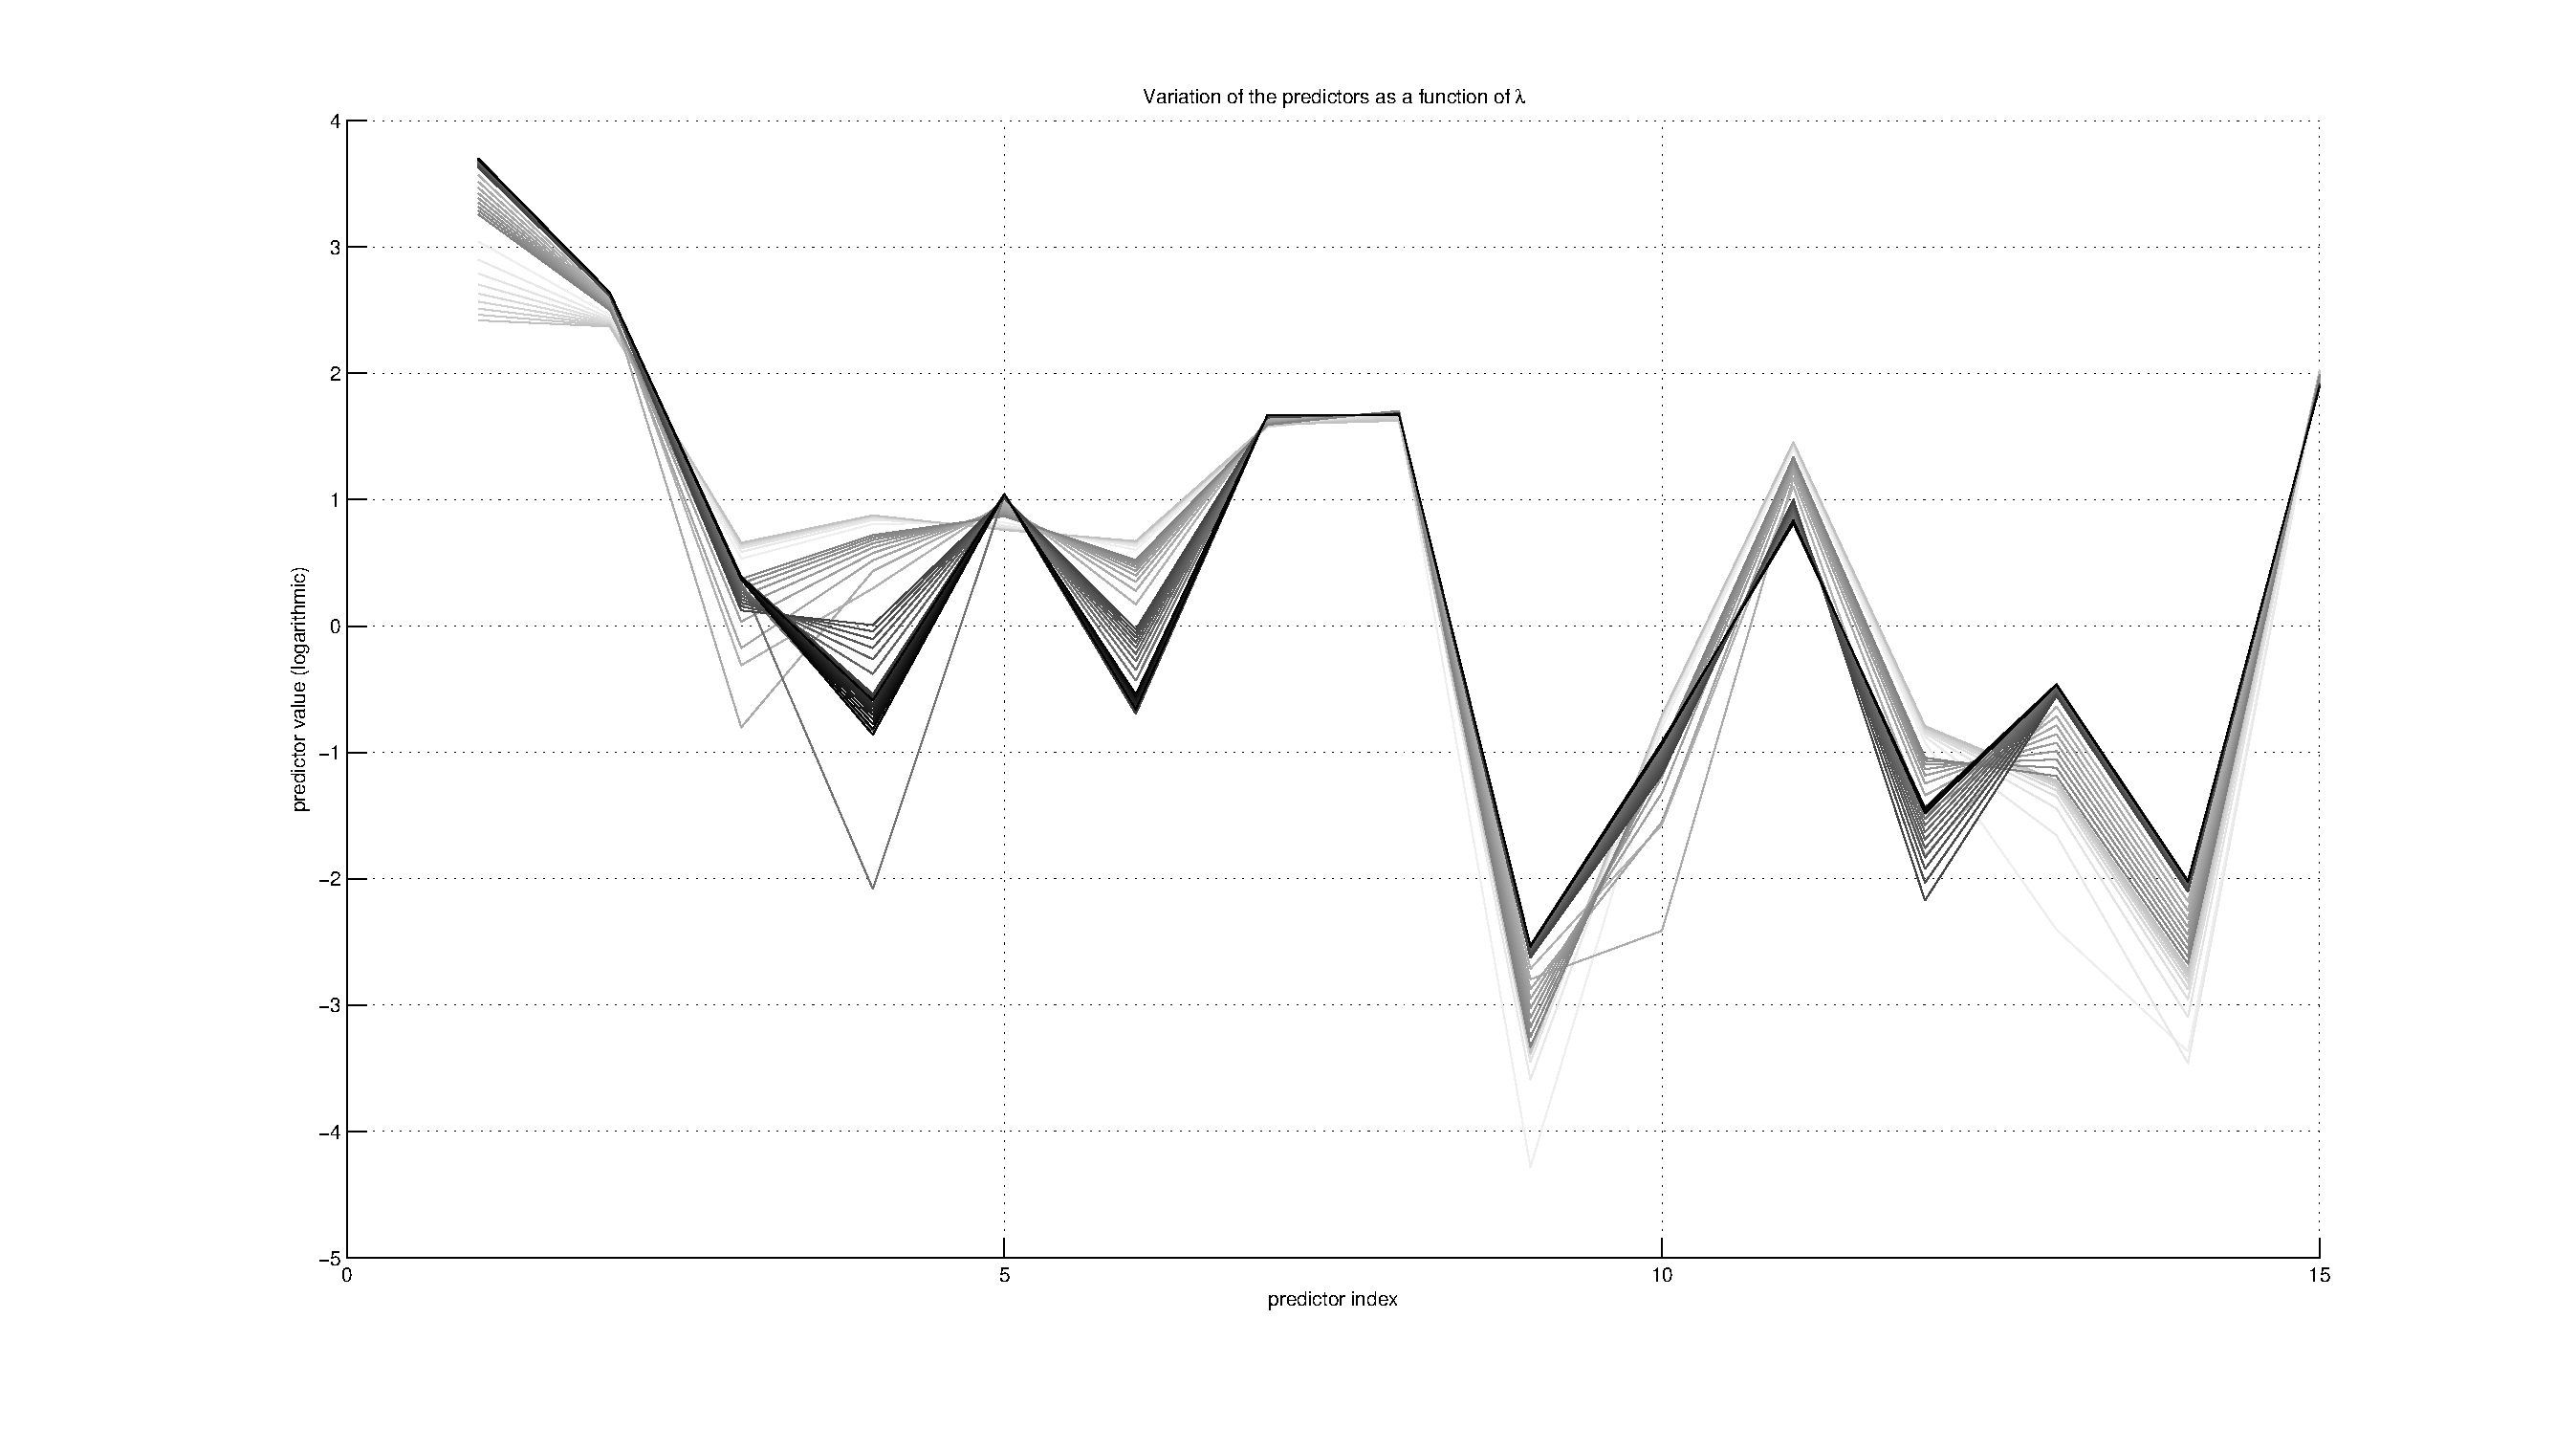
\includegraphics[width=0.75\textwidth]{../figures/PredictorsVsLambda.eps}
  \caption{Parameter evolution during prediction error minimization. Darker values are closer to the optimal $\lambda$.}
\end{figure}

\section{Features}
In a first step, we exponentiated some of the given features (e.g. $x_i \rightarrow x_i^a \text{ with } a \in [-2:0.5:5] \text{ and } a \neq 0$). \\
Next, we combined some of the transformed features in order to consider possible interactions. \\
Hence, our final model has the form $ y = \beta_0 + ... + \beta_i x_i^a + ... + \beta_z x_j^b x_k^c + ... $.

\section{Parameters}
\emph{Cross Validation} was used to find how to transform and combine the parameters. In details:
\begin{itemize}
\item For each feature $x_i$, the exponent $a$ is chosen so that the estimated prediction error is minimized.
\item For each pair of feature $x_i$ and $x_j$, the combination term $x_i x_j$ is included only if the estimated prediction error decreases by a certain percentage.  
\end{itemize}
\begin{figure}[h!]
        \centering
        \begin{subfigure}[b]{0.375\textwidth}
                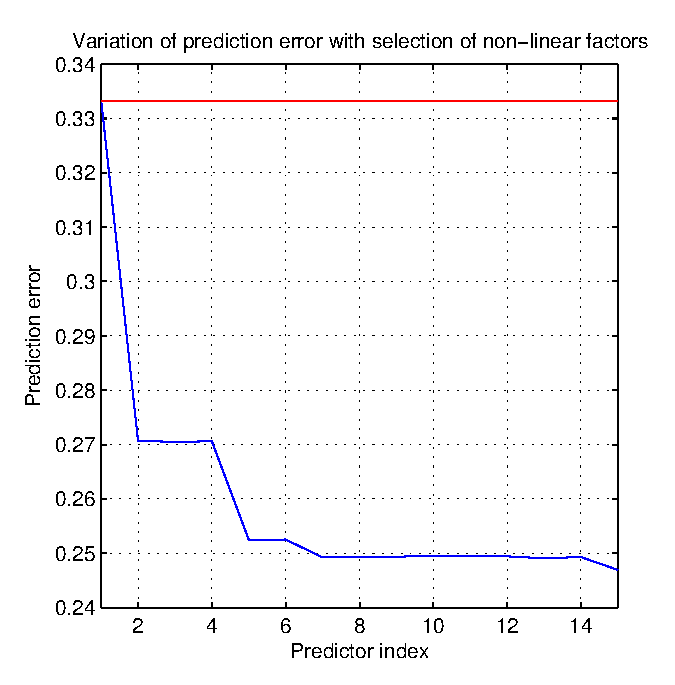
\includegraphics[width=\textwidth]{../figures/nonLinearFactors.eps}
                \label{fig:tiger}
        \end{subfigure}
        ~ %add desired spacing between images, e. g. ~, \quad, \qquad, \hfill etc.
          %(or a blank line to force the subfigure onto a new line)
        \begin{subfigure}[b]{0.375\textwidth}
                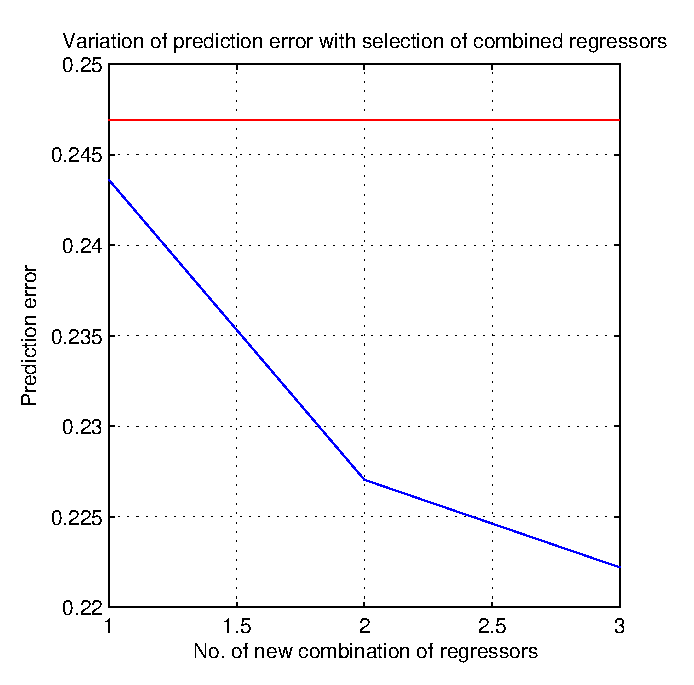
\includegraphics[width=\textwidth]{../figures/regressorCombination.eps}
                \label{fig:mouse}
        \end{subfigure}
        \caption{Error reduction through feature transformation and combination.}\label{fig:animals}
\end{figure}
\section{Lessons Learned} 
Other strategies that we tried include feature discarding\footnote{We computed the parameters $\beta$ on normalized data and excluded the features corresponding to the lowest $|\beta|$. }, response transformation and different feature transformations (e.g. $log(\cdot)$).
The resulting worse performance is most likely given by a loss of information (in the case of the discarded feature) or wrong model assumptions.

\end{document}
